\documentclass[11pt,a4paper]{article}

\usepackage[utf8]{inputenc}
\usepackage[T1]{fontenc}
\usepackage[spanish,es-tabla]{babel}
\usepackage{lmodern}
\usepackage[margin=2.5cm]{geometry}
\usepackage{graphicx}
\usepackage{booktabs}
\usepackage{amsmath}
\usepackage{listings}
\usepackage{xcolor}
\usepackage{float}
\usepackage[hidelinks]{hyperref}

\graphicspath{{figuras/}}

\lstset{
  basicstyle=\ttfamily\small,
  backgroundcolor=\color{gray!8},
  frame=single,
  rulecolor=\color{gray!40},
  breaklines=true,
  columns=fullflexible,
  keepspaces=true,
  literate={á}{{\'a}}1 {é}{{\'e}}1 {í}{{\'i}}1 {ó}{{\'o}}1 {ú}{{\'u}}1 {ñ}{{\~n}}1
           {→}{{$\rightarrow$}}1 {·}{{$\cdot$}}1
}

\title{Sistema de mapas de calor de goles\\
  \large RETO d/dx $\cdot$ MINUTO 90 --- Mundial Qatar 2022}
\author{Equipo SixSeven}
\date{\today}

\begin{document}

\maketitle

\begin{abstract}
Este reporte describe un sistema en Python que genera mapas de calor de goles y tiros
a partir de los datos de eventos del Mundial Qatar 2022 (StatsBomb Open Data).
El sistema lee la base SQLite del reto, transforma las coordenadas de cada tiro,
estima su densidad sobre la cancha y produce figuras listas para presentación,
ya sea de un partido o del torneo completo. Se documentan los datos, la arquitectura,
los métodos de estimación, el uso y los primeros resultados.
\end{abstract}

\tableofcontents

% ---------------------------------------------------------------------------
\section{Objetivo}

El reto pregunta \emph{qué pasa con los jugadores cuando el partido se decide}.
Un primer paso para responderla es ver \textbf{desde dónde} se anotan los goles:
qué zonas de la cancha concentran la definición, cómo cambia eso entre equipos
y en qué momento del partido ocurren. El sistema convierte la tabla de tiros
en un mapa de calor que responde la primera parte de forma visual y reproducible.

% ---------------------------------------------------------------------------
\section{Datos}

\subsection{Fuente}

Se usa el conjunto completo \texttt{RETO\_ddx\_MINUTO\_90\_completo}, en su versión
SQLite (\texttt{sql/minuto\_90.sqlite}). Cubre los 64 partidos del torneo,
32 selecciones y 680 jugadores, desde la fase de grupos hasta la final.
Las tablas de eventos provienen de StatsBomb Open Data (competición 43, temporada 106)
y fueron reorganizadas por NEXT LEVEL DX, que agregó las columnas \texttt{tramo}
y \texttt{estado\_marcador}.

\subsection{Tablas utilizadas}

\begin{table}[H]
\centering
\begin{tabular}{@{}llrl@{}}
\toprule
Tabla & Una fila es & Filas & Uso en el sistema \\
\midrule
\texttt{eventos\_tiros} & un tiro & 1\,453 & posición, minuto, equipo, resultado \\
\texttt{partidos}       & un partido & 64 & equipos, marcador y fase para el título \\
\bottomrule
\end{tabular}
\caption{Tablas de la base que consulta el sistema. Se unen por \texttt{match\_id}.}
\end{table}

De \texttt{eventos\_tiros} se usan las columnas \texttt{match\_id}, \texttt{minuto},
\texttt{equipo}, \texttt{rival}, \texttt{jugador}, \texttt{x}, \texttt{y}, \texttt{xg},
\texttt{gol} y \texttt{tipo\_tiro}. Un gol es una fila con \texttt{gol = 1}.

\subsection{Sistema de coordenadas}

La cancha mide $120 \times 80$ unidades (yardas). Todos los eventos están orientados
hacia el ataque del equipo que los realiza: $x = 0$ es su propia portería y
$x = 120$ la portería rival; $y = 0$ es la banda izquierda vista desde su portería.
Las áreas quedan en coordenadas fijas: el área grande va de $x = 102$ a $120$ y de
$y = 18$ a $62$; el punto penal está en $(108, 40)$.

\subsection{Consideraciones de calidad}

\begin{itemize}
  \item \textbf{Autogoles.} No son tiros, por lo que no aparecen en \texttt{eventos\_tiros}.
    La tabla registra 169 goles, mientras que la suma de marcadores en \texttt{partidos}
    es 172. Los tres faltantes son autogoles (Canada--Morocco, Costa Rica--Germany
    y Argentina--Australia). El sistema avisa cuando detecta esta diferencia.
  \item \textbf{Minuto.} Sigue la convención de StatsBomb y empieza en 0: un gol
    del minuto 80 de la transmisión se registra como 79.
  \item \textbf{Tandas de penales.} No están incluidas en la tabla de tiros, por lo
    que no se mezclan con los goles del partido.
  \item \textbf{Nombres.} Los equipos vienen en inglés. En las tablas usadas los
    nombres coinciden entre \texttt{eventos\_tiros} y \texttt{partidos}.
\end{itemize}

% ---------------------------------------------------------------------------
\section{Arquitectura del sistema}

El sistema es un solo script, \texttt{heatmap\_goles.py}, que depende de
\texttt{pandas}, \texttt{numpy} y \texttt{matplotlib}. El flujo es lineal:

\begin{enumerate}
  \item \textbf{Consulta.} \texttt{cargar\_tiros()} lee los tiros (o solo los goles)
    de un partido o del torneo; \texttt{cargar\_partido()} lee los datos del partido.
  \item \textbf{Transformación.} Se invierte el eje $Y$ (StatsBomb lo mide hacia abajo)
    y, cuando ambos equipos comparten la cancha, \texttt{reflejar()} gira 180° los tiros
    del visitante.
  \item \textbf{Densidad.} \texttt{densidad\_kde()} o \texttt{densidad\_zonas()} calculan
    la superficie a colorear.
  \item \textbf{Dibujo.} \texttt{dibujar\_cancha()} traza las líneas y
    \texttt{mapa\_de\_calor()} superpone la densidad, los tiros, las etiquetas y la
    barra de color.
  \item \textbf{Salida.} La figura se muestra en pantalla o se guarda en PNG, SVG o PDF.
\end{enumerate}

\begin{table}[H]
\centering
\begin{tabular}{@{}ll@{}}
\toprule
Función & Responsabilidad \\
\midrule
\texttt{listar\_partidos()}   & Imprime los 64 partidos con su \texttt{match\_id} \\
\texttt{cargar\_partido()}    & Fila de \texttt{partidos} para un \texttt{match\_id} \\
\texttt{cargar\_tiros()}      & Tiros o goles de un partido o del torneo \\
\texttt{densidad\_kde()}      & Densidad suavizada con kernel gaussiano \\
\texttt{densidad\_zonas()}    & Conteo en una cuadrícula de $12 \times 8$ \\
\texttt{dibujar\_cancha()}    & Líneas de la cancha en unidades StatsBomb \\
\texttt{mapa\_de\_calor()}    & Figura completa de un conjunto de tiros \\
\texttt{reflejar()}           & Giro de 180° para el equipo visitante \\
\texttt{graficar\_partido()}  & Vista de partido: una cancha o un panel por equipo \\
\texttt{avisar\_autogoles()}  & Compara goles registrados contra el marcador \\
\bottomrule
\end{tabular}
\caption{Funciones principales de \texttt{heatmap\_goles.py}.}
\end{table}

% ---------------------------------------------------------------------------
\section{Metodología}

\subsection{Densidad suavizada (modo \texttt{kde})}

Para cada punto $(x, y)$ de una malla con resolución de $0.5$ yardas se suma una
campana gaussiana centrada en cada tiro $(x_i, y_i)$:
\begin{equation}
  z(x, y) = \sum_{i=1}^{n} \exp\!\left( -\frac{(x - x_i)^2 + (y - y_i)^2}{2\sigma^2} \right),
  \qquad \sigma = 6 \text{ yardas}.
\end{equation}
Después se normaliza, $\hat z = z / \max z$, de modo que la escala va de 0 a 1 y
representa \emph{concentración relativa} dentro del mismo mapa; por eso la barra de
color se rotula ``Baja'' y ``Alta'' en lugar de un número absoluto. Los valores por
debajo de $0.05$ se dejan transparentes para que la cancha se siga viendo.

Se eligió un $\sigma$ generoso porque un partido suele tener entre 2 y 6 goles:
con un kernel estrecho cada gol sería una mancha aislada y el mapa no mostraría
zonas. La implementación es directa en \texttt{numpy}, sin depender de \texttt{scipy}.

\subsection{Conteo por zonas (modo \texttt{zonas})}

La cancha se divide en una cuadrícula de $12 \times 8$ celdas de $10 \times 10$ yardas y
se cuenta cuántos tiros caen en cada una (histograma 2D). Cada celda con al menos un
tiro muestra su conteo. Este modo es mejor cuando hay muchos goles, como en el torneo
completo, porque los números se pueden leer y comparar directamente.

\subsection{Orientación de los equipos}

En los datos ambos equipos atacan hacia $x = 120$. En la vista de un partido, el local
conserva su orientación y al visitante se le aplica $(x, y) \mapsto (120 - x,\ 80 - y)$,
de modo que cada equipo ataca una portería distinta y los dos caben en la misma cancha.
Con la opción \texttt{--por-equipo} no se gira a nadie: cada selección tiene su panel
atacando hacia la derecha, lo que facilita compararlas.

\subsection{Codificación visual}

\begin{itemize}
  \item Rampa secuencial de un solo tono (azul claro a oscuro): más oscuro significa más
    concentración. No se usa un arcoíris, que exagera diferencias pequeñas.
  \item Los goles se marcan como puntos negros con borde claro; con \texttt{--tiros}, los
    tiros fallados aparecen como círculos grises con relleno claro.
  \item Cada gol lleva su minuto. Los goles anotados desde el mismo punto (p.\ ej.\ penales)
    comparten una sola etiqueta. Con más de 15 goles no se escriben minutos.
  \item Cada figura incluye el crédito ``Datos: StatsBomb Open Data''.
\end{itemize}

% ---------------------------------------------------------------------------
\section{Uso}

Instalación:
\begin{lstlisting}
python -m venv .venv
source .venv/bin/activate
pip install -r requirements.txt
\end{lstlisting}

Ejemplos:
\begin{lstlisting}
python heatmap_goles.py --listar                        # ids de los partidos
python heatmap_goles.py --partido 3869685               # goles de la final
python heatmap_goles.py --partido 3869685 --por-equipo  # un panel por equipo
python heatmap_goles.py --partido 3869685 --tiros       # todos los tiros
python heatmap_goles.py --modo zonas                    # todo el torneo
python heatmap_goles.py --partido 3869685 --salida final.pdf
\end{lstlisting}

\begin{table}[H]
\centering
\begin{tabular}{@{}lp{10cm}@{}}
\toprule
Opción & Efecto \\
\midrule
\texttt{--listar}          & Lista los partidos con \texttt{match\_id}, fecha, fase y marcador. \\
\texttt{--partido ID}      & Partido a graficar; si se omite, todo el torneo. \\
\texttt{--modo kde|zonas}  & Mancha suavizada (por defecto) o conteo por cuadrícula. \\
\texttt{--por-equipo}      & Un panel por selección. \\
\texttt{--tiros}           & Incluye todos los tiros, no solo los goles. \\
\texttt{--salida ARCHIVO}  & Guarda la figura (PNG, SVG o PDF) en lugar de mostrarla. \\
\texttt{--db RUTA}         & Ruta alternativa a \texttt{minuto\_90.sqlite}. \\
\bottomrule
\end{tabular}
\caption{Opciones de línea de comandos.}
\end{table}

% ---------------------------------------------------------------------------
\section{Resultados}

\subsection{Caso: la final Argentina 3--3 France}

La figura~\ref{fig:final} muestra los seis goles de la final en una sola cancha.
Los de Argentina se reparten dentro del área, incluido el penal de Messi en el
minuto 22 (registrado como 22'). Dos de los tres goles de Francia salieron del
punto penal (79' y 117'), por lo que comparten etiqueta.

\begin{figure}[H]
  \centering
  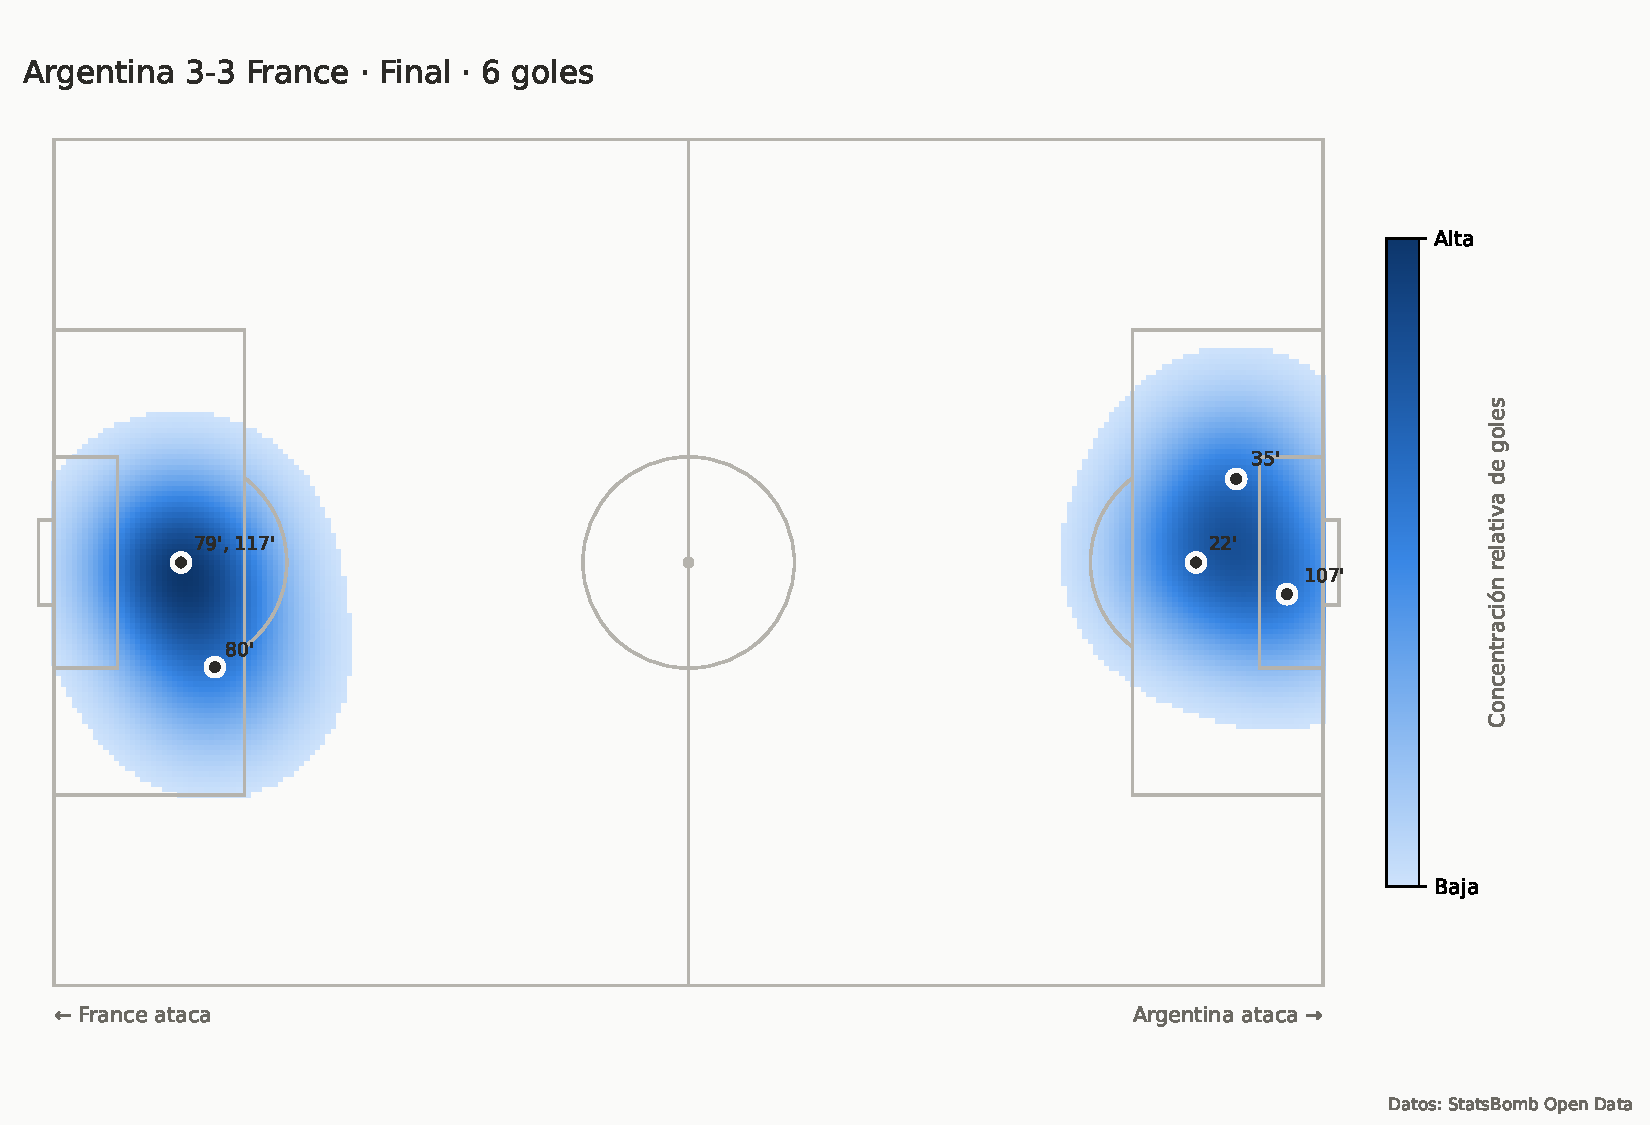
\includegraphics[width=\linewidth]{final_goles.pdf}
  \caption{Goles de la final. Argentina ataca a la derecha y Francia a la izquierda.}
  \label{fig:final}
\end{figure}

La figura~\ref{fig:final-tiros} agrega todos los tiros del partido. Argentina remató
20 veces y Francia 10; la mancha de Argentina es más amplia y se extiende fuera del
área, mientras que la de Francia se concentra en el borde del área.

\begin{figure}[H]
  \centering
  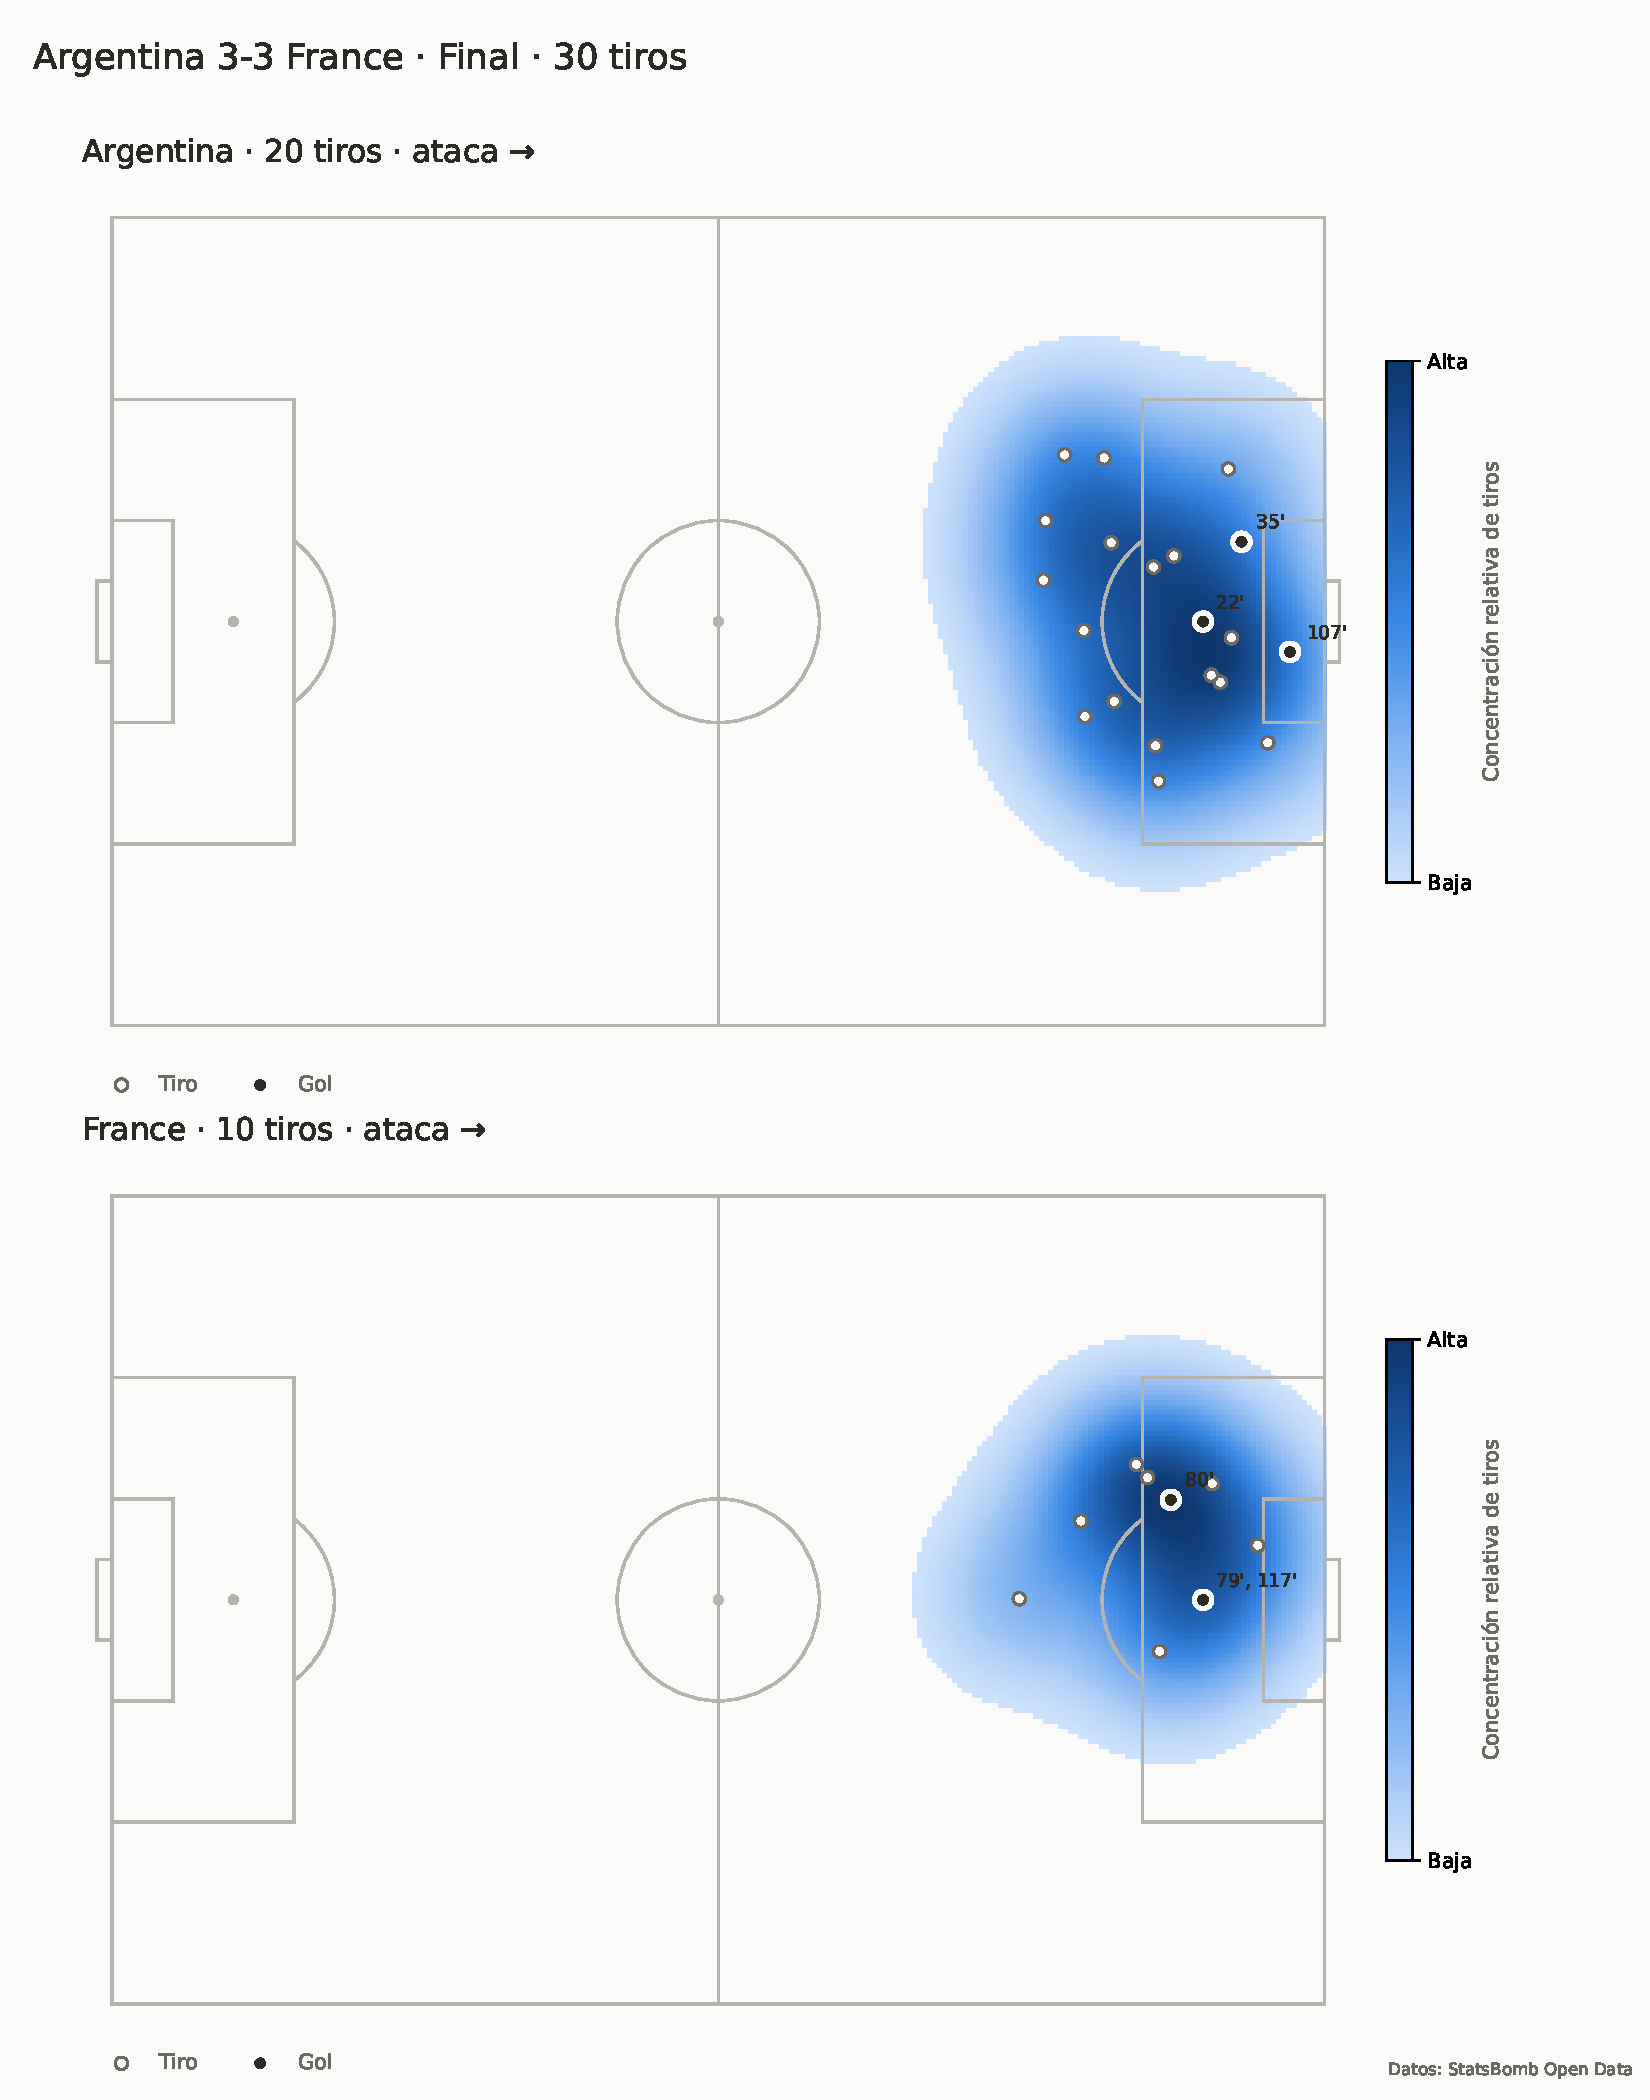
\includegraphics[width=0.85\linewidth]{final_tiros_equipo.pdf}
  \caption{Tiros de la final por equipo. Puntos negros: goles; círculos claros: tiros sin gol.}
  \label{fig:final-tiros}
\end{figure}

\subsection{Torneo completo}

\begin{table}[H]
\centering
\begin{tabular}{@{}lr@{}}
\toprule
Indicador & Valor \\
\midrule
Tiros registrados                        & 1\,453 \\
Goles (sin autogoles)                    & 169 \\
Conversión (goles / tiros)               & 11.6\,\% \\
Goles desde dentro del área grande       & 92.9\,\% \\
Goles desde el área chica                & 19.5\,\% \\
Tiros desde dentro del área grande       & 62.7\,\% \\
Distancia media del gol a la portería    & 12.3 yardas \\
xG medio de los tiros que fueron gol     & 0.31 \\
Goles de penal                           & 17 \\
Goles de tiro libre directo              & 2 \\
\bottomrule
\end{tabular}
\caption{Resumen de tiros y goles del Mundial 2022.}
\label{tab:resumen}
\end{table}

La figura~\ref{fig:torneo} confirma lo que muestra la tabla~\ref{tab:resumen}: casi todos los
goles nacen dentro del área, y las dos celdas frente a la portería concentran 78 de los 169.
Aunque solo el 62.7\,\% de los tiros se hacen dentro del área, de ahí sale el 92.9\,\% de los goles.

\begin{figure}[H]
  \centering
  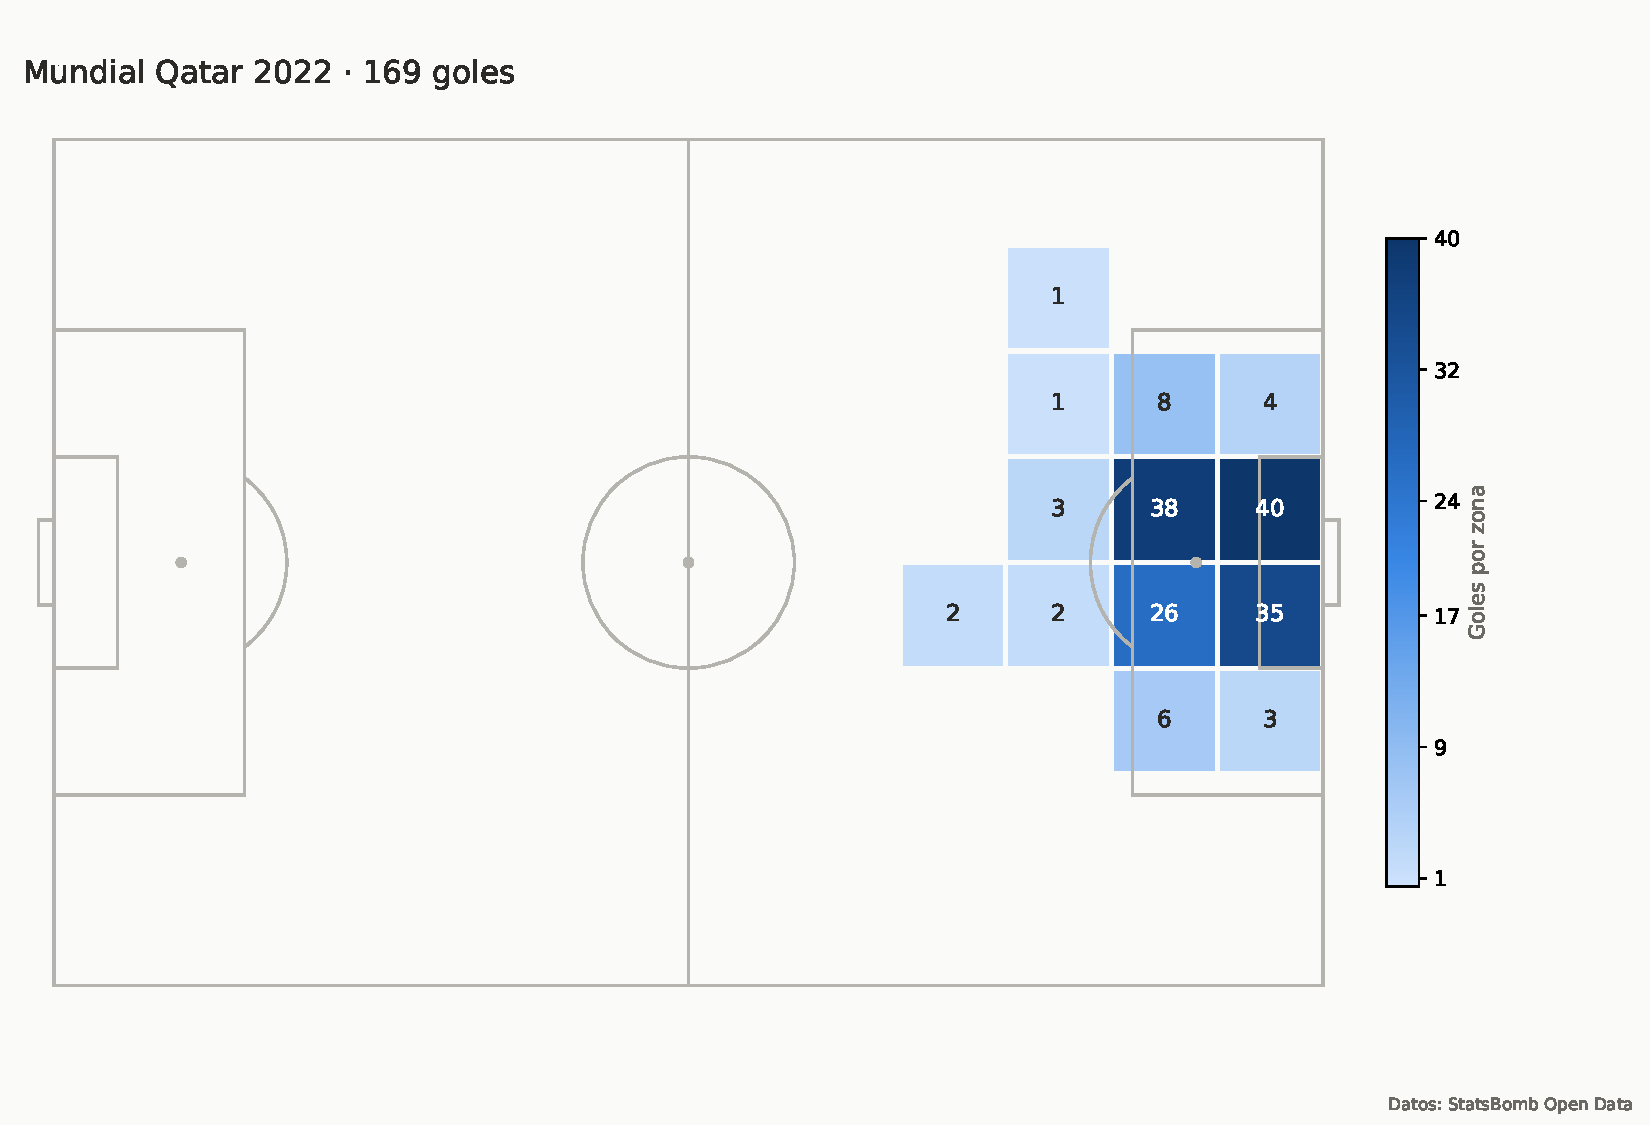
\includegraphics[width=\linewidth]{torneo_zonas.pdf}
  \caption{Goles del torneo por zonas de $10 \times 10$ yardas.}
  \label{fig:torneo}
\end{figure}

\begin{figure}[H]
  \centering
  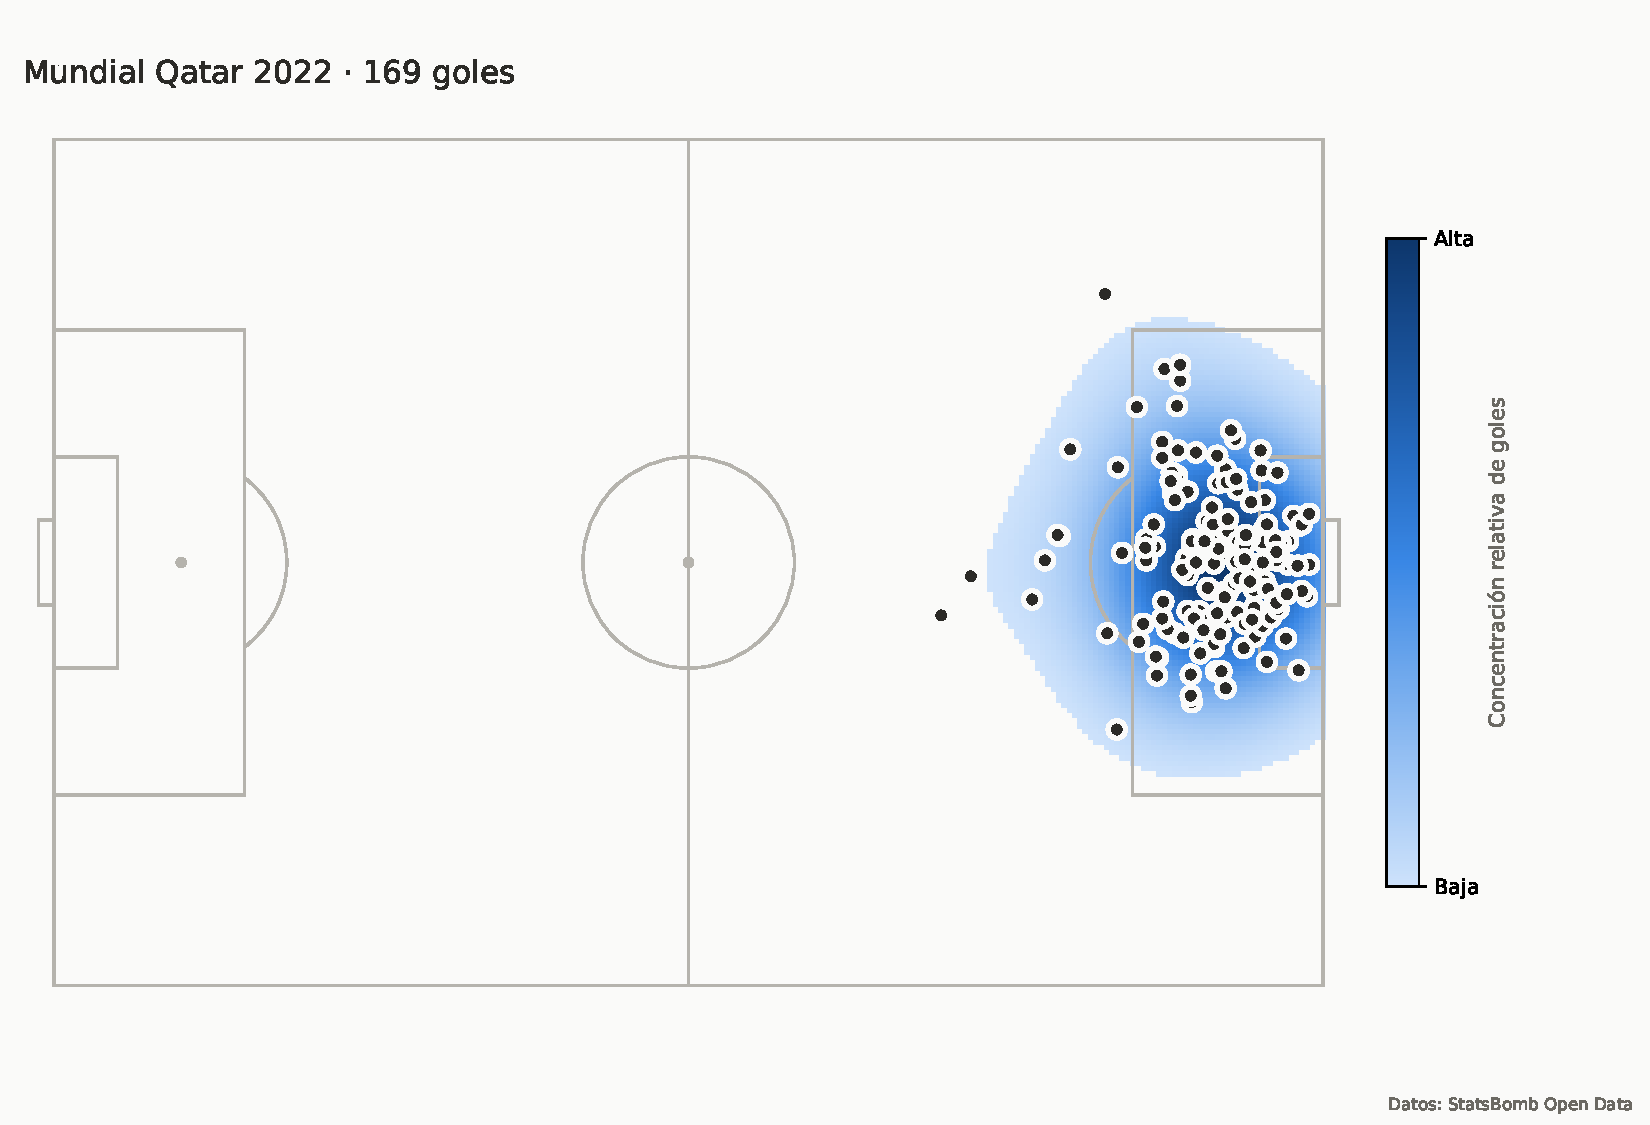
\includegraphics[width=\linewidth]{torneo_kde.pdf}
  \caption{Densidad suavizada de los 169 goles del torneo.}
  \label{fig:torneo-kde}
\end{figure}

\subsection{¿Cuándo se anotan?}

Ligado a la pregunta del reto, la columna \texttt{tramo} muestra que el cierre del partido
es el bloque de 15 minutos con más goles (tabla~\ref{tab:tramos}).

\begin{table}[H]
\centering
\begin{tabular}{@{}lr@{}}
\toprule
Tramo & Goles \\
\midrule
00--15     & 15 \\
15--30     & 16 \\
30--45     & 30 \\
45+ (1T)   & 5 \\
45--60     & 28 \\
60--75     & 30 \\
75--90+    & \textbf{41} \\
Prórroga   & 4 \\
\bottomrule
\end{tabular}
\caption{Goles por tramo de 15 minutos. El tramo 75--90+ incluye el tiempo añadido del segundo tiempo.}
\label{tab:tramos}
\end{table}

% ---------------------------------------------------------------------------
\section{Limitaciones y trabajo futuro}

\begin{itemize}
  \item Los autogoles no se pueden ubicar porque no hay tiro asociado.
  \item La densidad está normalizada por figura, así que dos mapas no son comparables en
    intensidad absoluta; para comparar equipos conviene el modo \texttt{zonas}.
  \item Pendiente: filtrar por \texttt{tramo} y \texttt{estado\_marcador} para responder
    directamente cómo cambia la definición en el cierre del partido o cuando se va perdiendo.
  \item Pendiente: ponderar la densidad por \texttt{xg} para mapear calidad de las ocasiones
    y no solo su cantidad.
  \item Pendiente: mapas de calor de \texttt{eventos\_acciones} (229\,319 acciones) para ver
    la actividad de un jugador en todo el campo.
\end{itemize}

% ---------------------------------------------------------------------------
\section*{Créditos}

Datos: StatsBomb Open Data, reorganizados por NEXT LEVEL DX para el RETO d/dx.
Uso exclusivo para el reto; los datos deben borrarse a más tardar el 31 de octubre de 2026.

\end{document}
